\documentclass[
 paper=A4,pagesize=automedia,fontsize=12pt,
 BCOR=15mm,DIV=22,
 twoside,headinclude,footinclude=false,
 fleqn,                     % fleqn = linksbündige Ausrichtung von Formeln
 bibtotocnumbered,          % Literaturverz. im Inhaltsverz. eintragen
 liststotoc,                % Abbildungsverz. im Inhaltsverz. eintragen
 listsleft,                 % Abbildungsverz. an der längsten Nummer ausrichten
 %pointlessnumbers,          % kein Punkt nach Überschriftsnummerierung
 cleardoublepage=empty      % Vakatseiten ohne Paginierung
]{scrbook}
\setlength\parindent{0em}

% Kodierung, Schrift und Sprache auswählen
\usepackage[utf8]{inputenc}
\usepackage[T1]{fontenc}
\usepackage{babel}
% damit man Text aus dem PDF korrekt rauskopieren kann
\usepackage{cmap}
% Layout: Kopf-/Fußzeilen, anderthalbfacher Zeilenabstand
\usepackage{scrpage2} \pagestyle{scrheadings}
                      \clearscrheadfoot
                      \ihead{\headmark}\ohead{\pagemark}
                      \automark[subsection]{section}
                      \setheadsepline{0.5pt}
\usepackage{setspace} \onehalfspacing
\deffootnote{1em}{1em}{\textsuperscript{\thefootnotemark }}
% Grafiken, Tabellen, Mathematikumgebungen
\usepackage{graphicx,xcolor}
\usepackage{tabularx}
\usepackage{amsmath,amsfonts,amssymb}
% Darstellung von Fließumgebungen
\usepackage{flafter,afterpage}
\usepackage[section]{placeins}
\usepackage[margin=8mm,font=small,labelfont=bf,format=plain]{caption}
\usepackage[margin=8mm,font=small,labelfont=bf,format=plain]{subcaption}

\numberwithin{equation}{chapter}
\numberwithin{figure}{chapter}
\numberwithin{table}{chapter}

%%%%%%%%%%%%%%%%%%%%%%%%%%%%%%%%%%%%%%%%%%%%%%%%%%%%%%%%%%%%%%%%%%%%%%%%%%%%%%%%
% Ab hier ist Platz für eigene Ergänzungen (Pakete, Befehle, etc.)

% Dieses Paket liefert den Blindtext, der als Platzhalter in den Beispieldateien steht.
% Das kannst Du also entfernen, wenn Du den Blindtext nicht mehr brauchst.
\usepackage{lipsum}
%\usepackage{ bbold }
\usepackage{physics}
\usepackage{svg}
\usepackage{yfonts}
\usepackage{dsfont}
\begin{document}

\frontmatter


% Titelpageseite
\begin{titlepage}
 \begin{tabularx}{\linewidth}{X}
  
\includegraphics[width=6cm]{TU_Logo_SW} \\\hline\hline

  \vspace{4.5em}

  \begin{singlespace}\begin{center}\bfseries\Huge
  
  Title of Bachelor thesis
  
  \end{center}\end{singlespace}

  \vspace{5.5em}

  \begin{singlespace}\begin{center}\large
   Bachelor-Arbeit \\ zur Erlangung des Hochschulgrades \\ 
   Bachelor of Science \\ 
   im Bachelor-Studiengang Physik
  \end{center}\end{singlespace}\medskip

  \begin{center}vorgelegt von\end{center}
  \begin{center}
   {\large Felix Soest} \\ geboren am 16.09.1998 in Düsseldorf
  \end{center}\medskip

  \begin{singlespace}\begin{center}\large
   Institut für Theoretische Physik \\
   Fakultät Physik \\
   Bereich Mathematik und Naturwissenschaften \\
   Technische Universität Dresden \\ 2021
  \end{center}\end{singlespace}
 \end{tabularx}
\end{titlepage}


% Gutachterseite
\thispagestyle{empty}\vspace*{48em}

Eingereicht am xx.~Monat~20xx\vspace{1.5em}
\par{\large\begin{tabular}{ll}
 1. Gutachter: & Prof.~Dr.~Walter Strunz \\
 2. Gutachter: & Associate Professor Oscar Dahlsten, Ph.D. \\
\end{tabular}}


% Abstractseite
\newpage
\begin{center}\large\bfseries Summary\end{center}


Abstract \\ 
English: \\
Aufmerksamkeit
große Fragen?
unsere Frage
unsere Antwort

\vspace{20em}
Abstract \\ 
Deutsch \\
 
 
% Inhaltsverzeichnis
%\cleardoublepage
\tableofcontents



% Hauptteil
\mainmatter

\chapter{Introduction}
\lipsum
\section{Intro}
% !TeX root = ../BA_main_englisch.tex
% !TeX spellcheck = en_GB
Thermodynamics has been a central field of interest in physics ever since its inception in the 19th century \cite{thomson_2011}.

Due to the increasing availability of data and computing power, machine learning methods have become a standard approach in many fields such as natural language processing \cite{DBLP:journals/corr/VaswaniSPUJGKP17}.
Additionally, these methods are being applied to a broad range of problems in the physical sciences, from statistical physics to quantum computing \cite{Carleo_2019, wise2021using}.

Machine learning has also found use in the field of energy harvesting, concerned with extracting energy from external excitations, e.g. vibrations in human motion \cite{Liu2019}.
In this work we extend this concept to the quantum case.
Work extraction is often modelled as a system coupled to a heat bath, and bounds for the extractable work exist \cite{Egloff_2015}.
We take a different approach, following the framework given in \cite{beyer2020}.
We examine a system that can be driven by an arbitrary excitation, modelled as a time-dependent system Hamiltonian.
The transducer is modelled in a similar fashion and can extract work from the system.
By following a policy of local optimisation of the work output, we show that a lower bound of the extractable work exists for specific initial conditions.
We train neural networks to predict transducer protocols given a drive sequence, considering both the case where the sequence is known beforehand and the one where it is not.

The remainder of this work is structured as follows.
In Chapter \ref{background} we review the collision model framework used in our approach and introduce two machine learning architectures.
In Chapter \ref{lower_bound} we show that for a given drive sequence a lower bound on the expectation value of the extractable work exists.
We investigate the system under consideration in Section \ref{dep_dt} and apply the aforementioned architectures in Sections \ref{n_2_ml} to \ref{work_cost}.
We summarise our findings and provide an outlook in Chapter \ref{outlook}.

We use units where $\hbar = 1$.

\chapter{Background}


\section{Supervised Machine Learning}
Machine learning is a subfield of artificial intelligence, `concerned with the question of how to construct computer programs that automatically improve with experience.' \cite{Mitchell97}
Supervised machine learning is one of the three machine learning disciplines, besides unsupervised and reinforcement learning.
The goal is to find a mapping between an input and an output, in our case an excitation and its respective optimal harvesting policy.
Multiple algorithms to find such a mapping exist, however for high dimensional problems artificial neural networks (ANNs) are usually used.
In the following sections we review two ANN architectures, the fully-connected feedforward ANN and the Long Short-Term Memory (LSTM) network.

\subsection{Fully-connected feedforward ANNs}
In this section we review ANNs, following the exposition given in \cite{lu2020dying}.
Let $\textfrak{N}$ be a fully-connected feedforward ANN, meaning there are no loops in the neuron connections and all neurons in a layer are connected to every neuron of the next layer, $\textfrak{N}: \mathbb{R}^{n_1} \to \mathbb{R}^{n_L}$. $n_1$ and $n_L$ denote the dimensionality of the input and output respectively. 
$\textfrak{N}$ has $L$ layers, or columns of neurons.
The network architecture is given by the amount of neurons $n_l$ in each hidden layer $l \in [2, L - 1]$ (see figure \ref{nn}).
The neurons in layer $l$ are represented by their activations $\vec{a}_l \in \mathbb{R}^{n_l}$, which represent the matrix multiplication output. Additionally each layer includes trainable parameters $W_l \in \mathbb{R}^{n_{l+1} \times n_{l}}$ and $\vec{b}_l \in \mathbb{R}^{n_l}$ called weights and biases.
The activations can then be calculated using the following formulae \cite{TN_libero_mab2)53517}:
\begin{align*}
	\vec{a}_2 & = W_1 \vec{a}_1 + \vec{b}_1, \\
	\vec{a}_l & = W_{l-1} \xi(\vec{a}_{l-1}) + \vec{b}_{l-1}, \ l \in [3, L],
\end{align*}
where $\xi(x)$ is a function called the activation function applied elementwise. Historically, functions such as $\tanh$ and sigmoid have been used. However, it has been shown \cite{Maas2013RectifierNI, krizhevsky} that the rectified linear unit $\mathrm{ReLU}(x) = \mathrm{max}(0, x)$ often provides better results and is used here.


\subsection{Long Short-Term Memory}
While the network architecture introduced in the previous section performs reasonably well on many problems, it destroys spatial and temporal correlations present in the data. 
Instead convolutional and recurrent networks are often used for these purposes, e.g. in image recognition and time series forecasting \cite{rumelhart1986learning, 10.1007/978-3-642-46466-9_18}.

Here we use the LSTM architecture, a type of recurrent neural network (RNN) introduced in \cite{doi:10.1162/neco.1997.9.8.1735}. 
The core idea of RNNs is the usage of loops to store and propagate information through time.

The network is made up of a row of LSTM cells which share parameters.
The cell uses the current input $x_t$ as well as the previous cell state $c_{t-1}$ and output $h_{t-1}$ to compute the output $h_t$.
Internally, the cell is comprised of multiple gates which control the storage of information, $i_t, f_t, g_t, o_t$, which are the input, forget, cell and output gates respectively.
The output and gates of each cell are computed using the following equations:
\begin{align*}
i_t & = \sigma (W_{ii} x_t + b_{ii} + W_{hi} h_{t-1} + b_{hi}), \\
f_t & = \sigma (W_{if} x_t + b_{if} + W_{hf} h_{t-1} + b_{hf}), \\
g_t & = \tanh (W_{ig} x_t + b_{ig} + W_{hg} h_{t-1} + b_{hg}), \\ 
o_t & = \sigma (W_{if} x_t + b_{if} + W_{hf} h_{t-1} + b_{hf}), \\
c_t & = f_t \odot c_{t-1} + i_t \odot g_t, \\
h_t & = o_t \odot \tanh (c_t).
\end{align*}

\subsection{Training \& Backpropagation}
To train an ANN a cost function is defined, often the mean squared error 
\begin{align*}
	\mathrm{MSE} = \frac{1}{N} \sum_{i=1}^N (\vec{a}_{L, i} - \vec{y}_i)^2,
\end{align*}
where the summation is performed over the training data $\{(\vec{x}_i, \vec{y}_i)\}$ with $N$ samples, where $\{\vec{x_i}\}$ is the input and $\{\vec{y_i}\}$ the output data, and $\vec{a}_{L, i} = \textfrak{N}(\vec{x}_i)$ is the output of the neural network.
The so-called backpropagation algorithm is used to calculate the gradient of the cost function with respect to the trainable parameters and improve the performance of the ANN \cite{rumelhart1986learning, nielsenneural}.

\begin{figure}
	\centering
	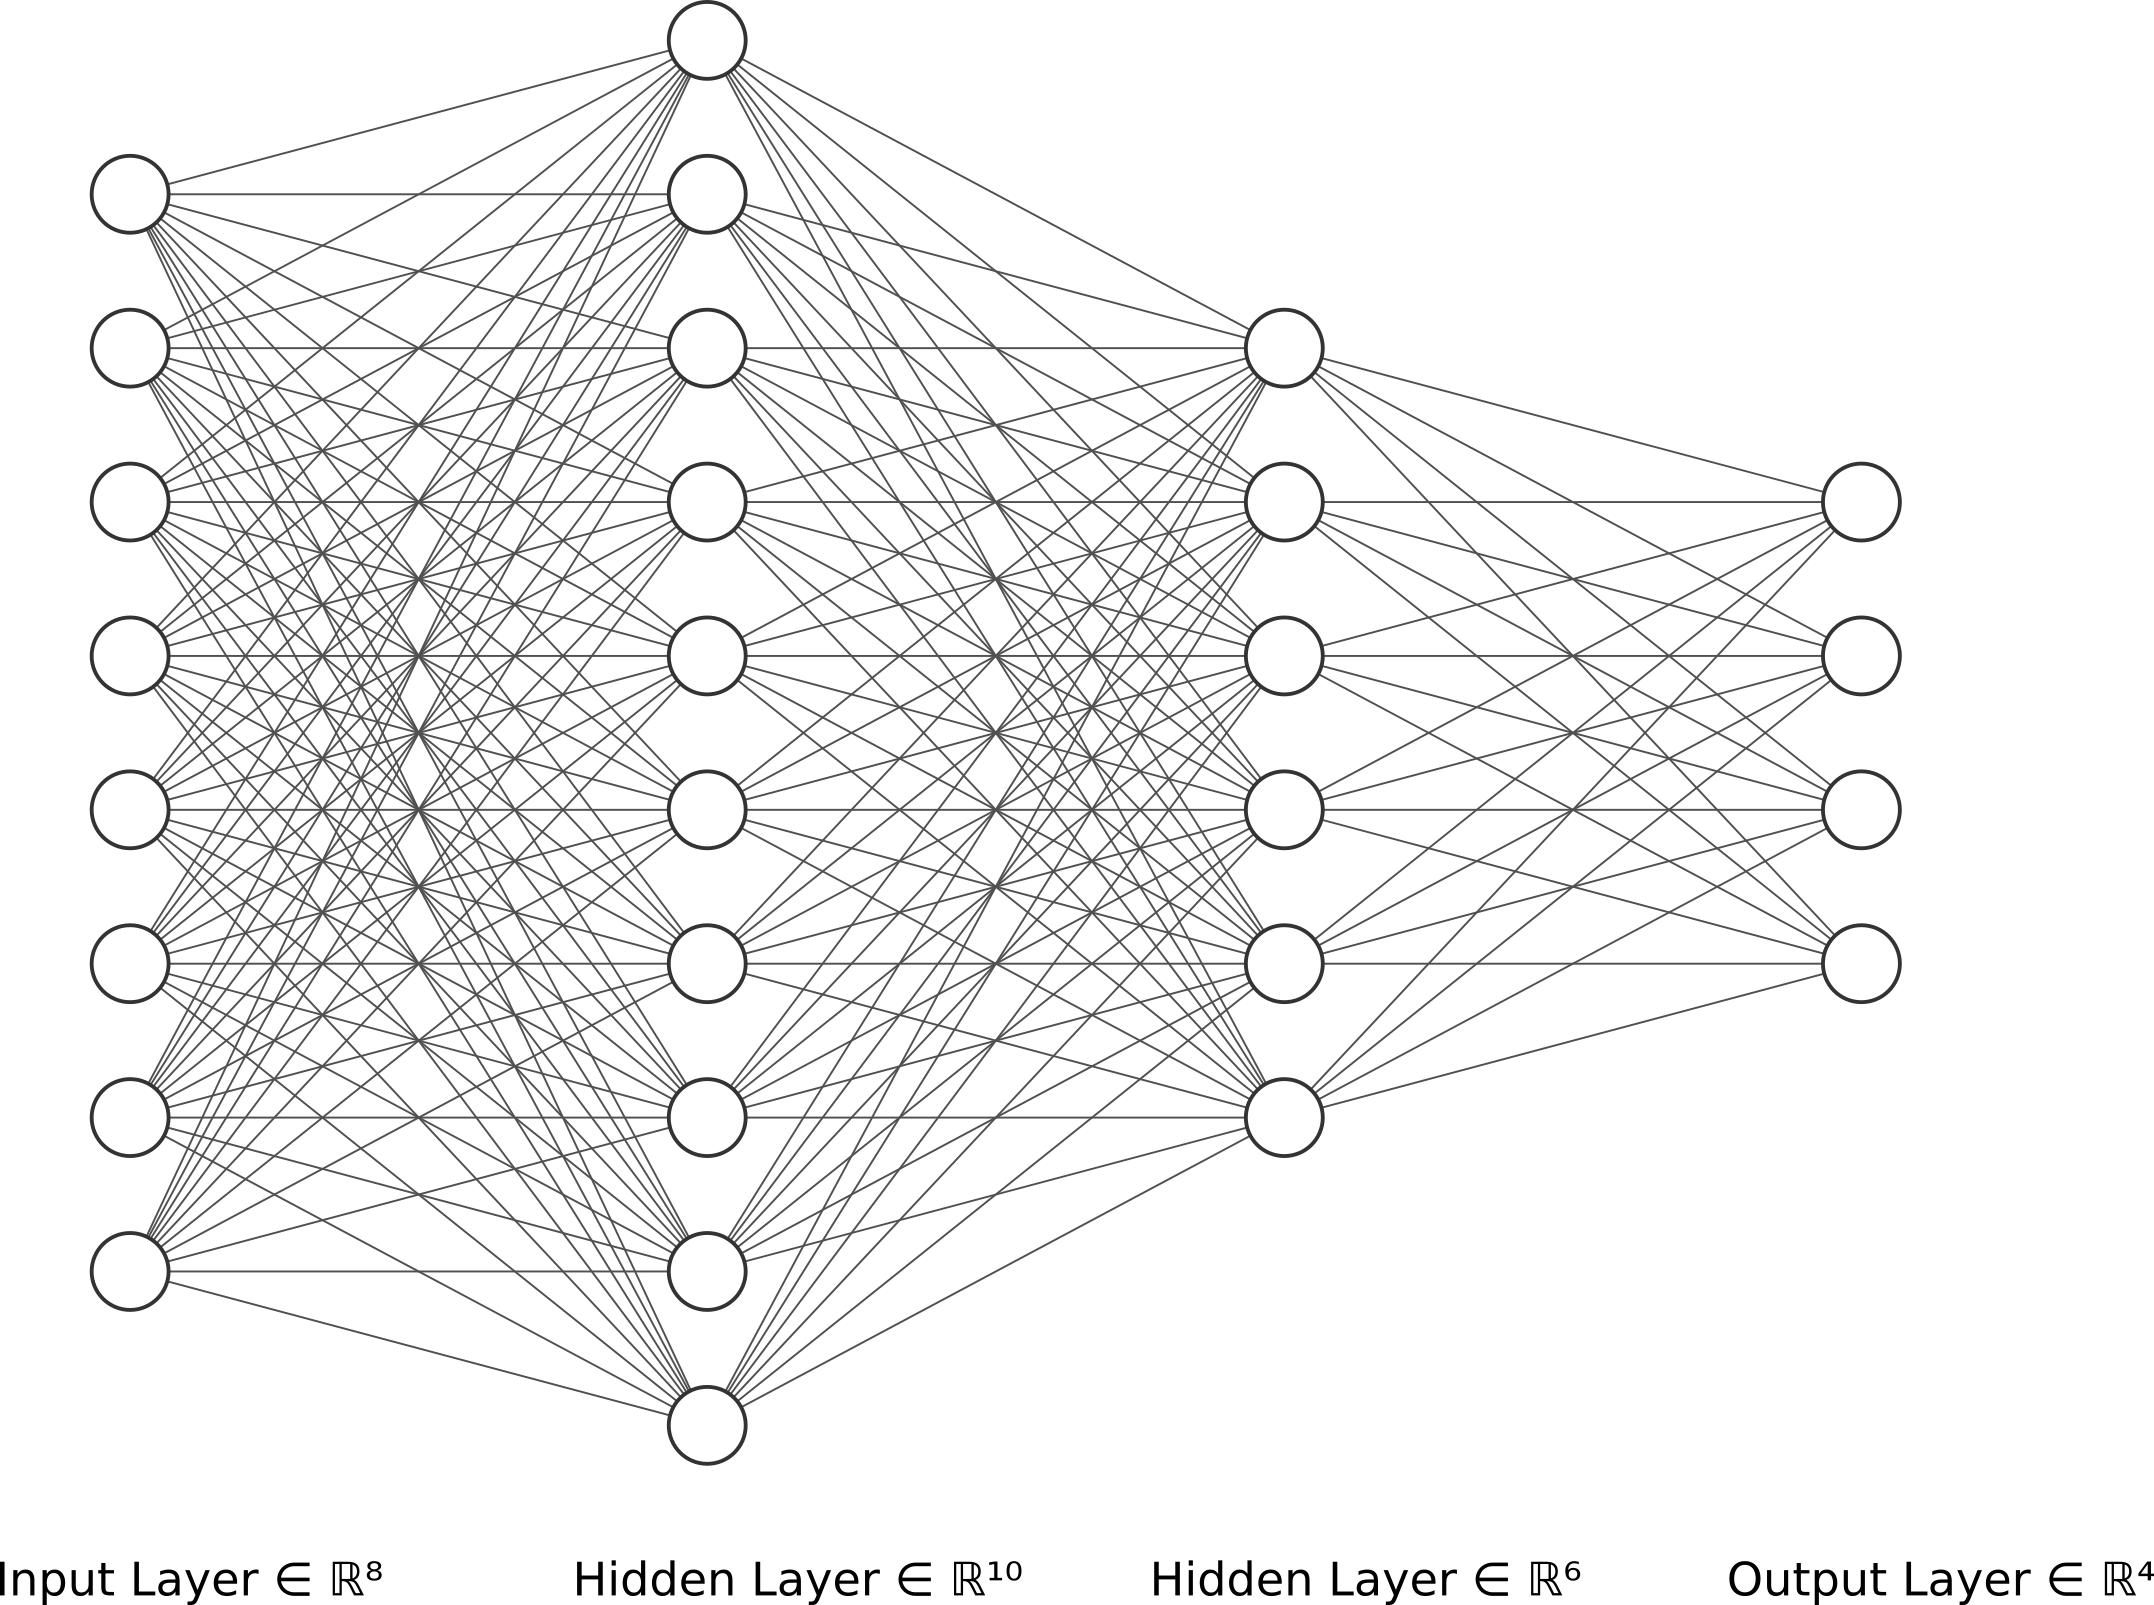
\includegraphics[width=0.6\textwidth]{img/nn}
	\caption{Example fully-connected feedforward ANN with four layers, including input, output and two hidden layers \cite{LeNail2019}}.
	\label{nn}
\end{figure}



\section{Setting}
Our setting consists of three qubits: the Drive, System and Transducer qubits. The Drive and Transducer qubits can be set by the experimenter in N discrete steps modelled as piecewise constant functions (PWC) of ($\theta_D, \phi_D$) and ($\theta_T, \phi_T$) respectively (see figure \ref{pwc}), the system qubit is initialised in a pure state.
As Drive and Transducer are assumed to be piecewise constant and therefore pure, we model both qubits as ancillary systems introduced in section \ref{col_model} (see figure \ref{collmodel}).

In the remainder of this work we use the interaction Hamiltonian on the three qubit Hilbert space
\begin{equation*}
	H_{DST} = H_{I} \otimes \mathds{1}_T + \mathds{1}_D \otimes H_{I}, \\
	H_{I} = \sigma_{+} \otimes \sigma_{-} + \sigma_{-} \otimes \sigma_{+}
\end{equation*}
unless otherwise noted.
The time evolution and work extraction is then calculated as follows, where $\Delta \mathrm{T}$ is time span between qubit switching\footnote{It is important to make the distinction between $\Delta \mathrm{T}$ and $\Delta t$ introduced in section \ref{col_model}. $\Delta t$ is the collision time of a single qubit while $\Delta \mathrm{T}$ is the time for which the qubits have the same initial state. For each time step $i$ we therefore have $n = \Delta \mathrm{T} / \Delta t$ qubits initialised in the same state.}:
\begin{align}
	H_S^i = \bra{\psi_D^i}\bra{\psi_T^i} H_{DST} \ket{\psi_D^i} \ket{\psi_T^i} \\
	\rho_S^{i+1} = U^i \rho_S^i U^{i\dagger}, \ U^i = e^{-iH_S^i \Delta \mathrm{T}} \\
	W = - \Sigma_i \mathrm{Tr} \ \rho_S^i \ dH_S^i \\
	dH_S^i = \bra{\psi_D^i}\bra{\psi_T^{i+1}} H_{DST} \ket{\psi_D^i} \ket{\psi_T^{i+1}} - \bra{\psi_D^i}\bra{\psi_T^i} H_{DST} \ket{\psi_D^i} \ket{\psi_T^i}.	
\end{align}
Here we use the partial Hamiltonian $H_S^i$ on S at time step $i \in [1, N - 1]$, as well as corresponding system density matrix $\rho_S^i$.


\begin{figure}
	\centering
	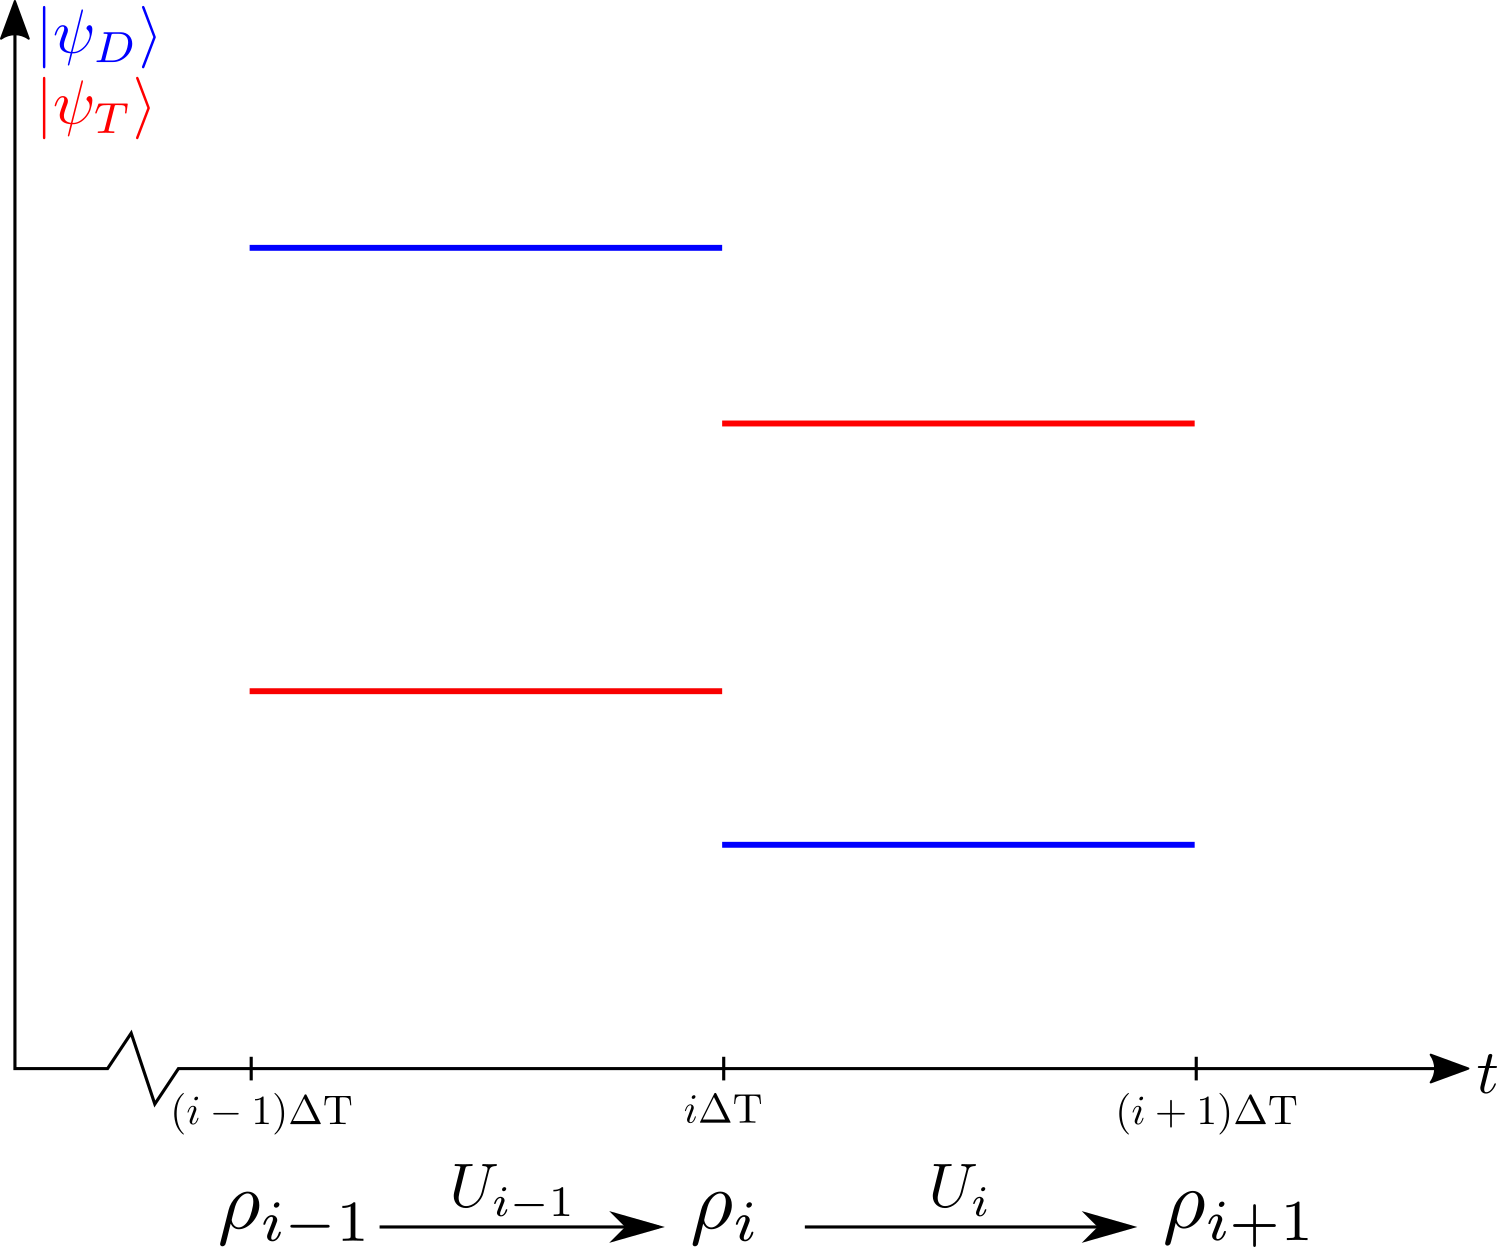
\includegraphics[width=0.6\textwidth]{img/pwc}
	\caption{Piecewise constant implementation of Drive and Transducer qubits: the vertical axis shows qubit state in arbitrary units. The qubit states are switched instantaneously and then kept constant for $\Delta \mathrm{T}$ while $\rho_S$ evolves unitarily.}
	\label{pwc}
\end{figure}

\begin{figure}
	\centering
	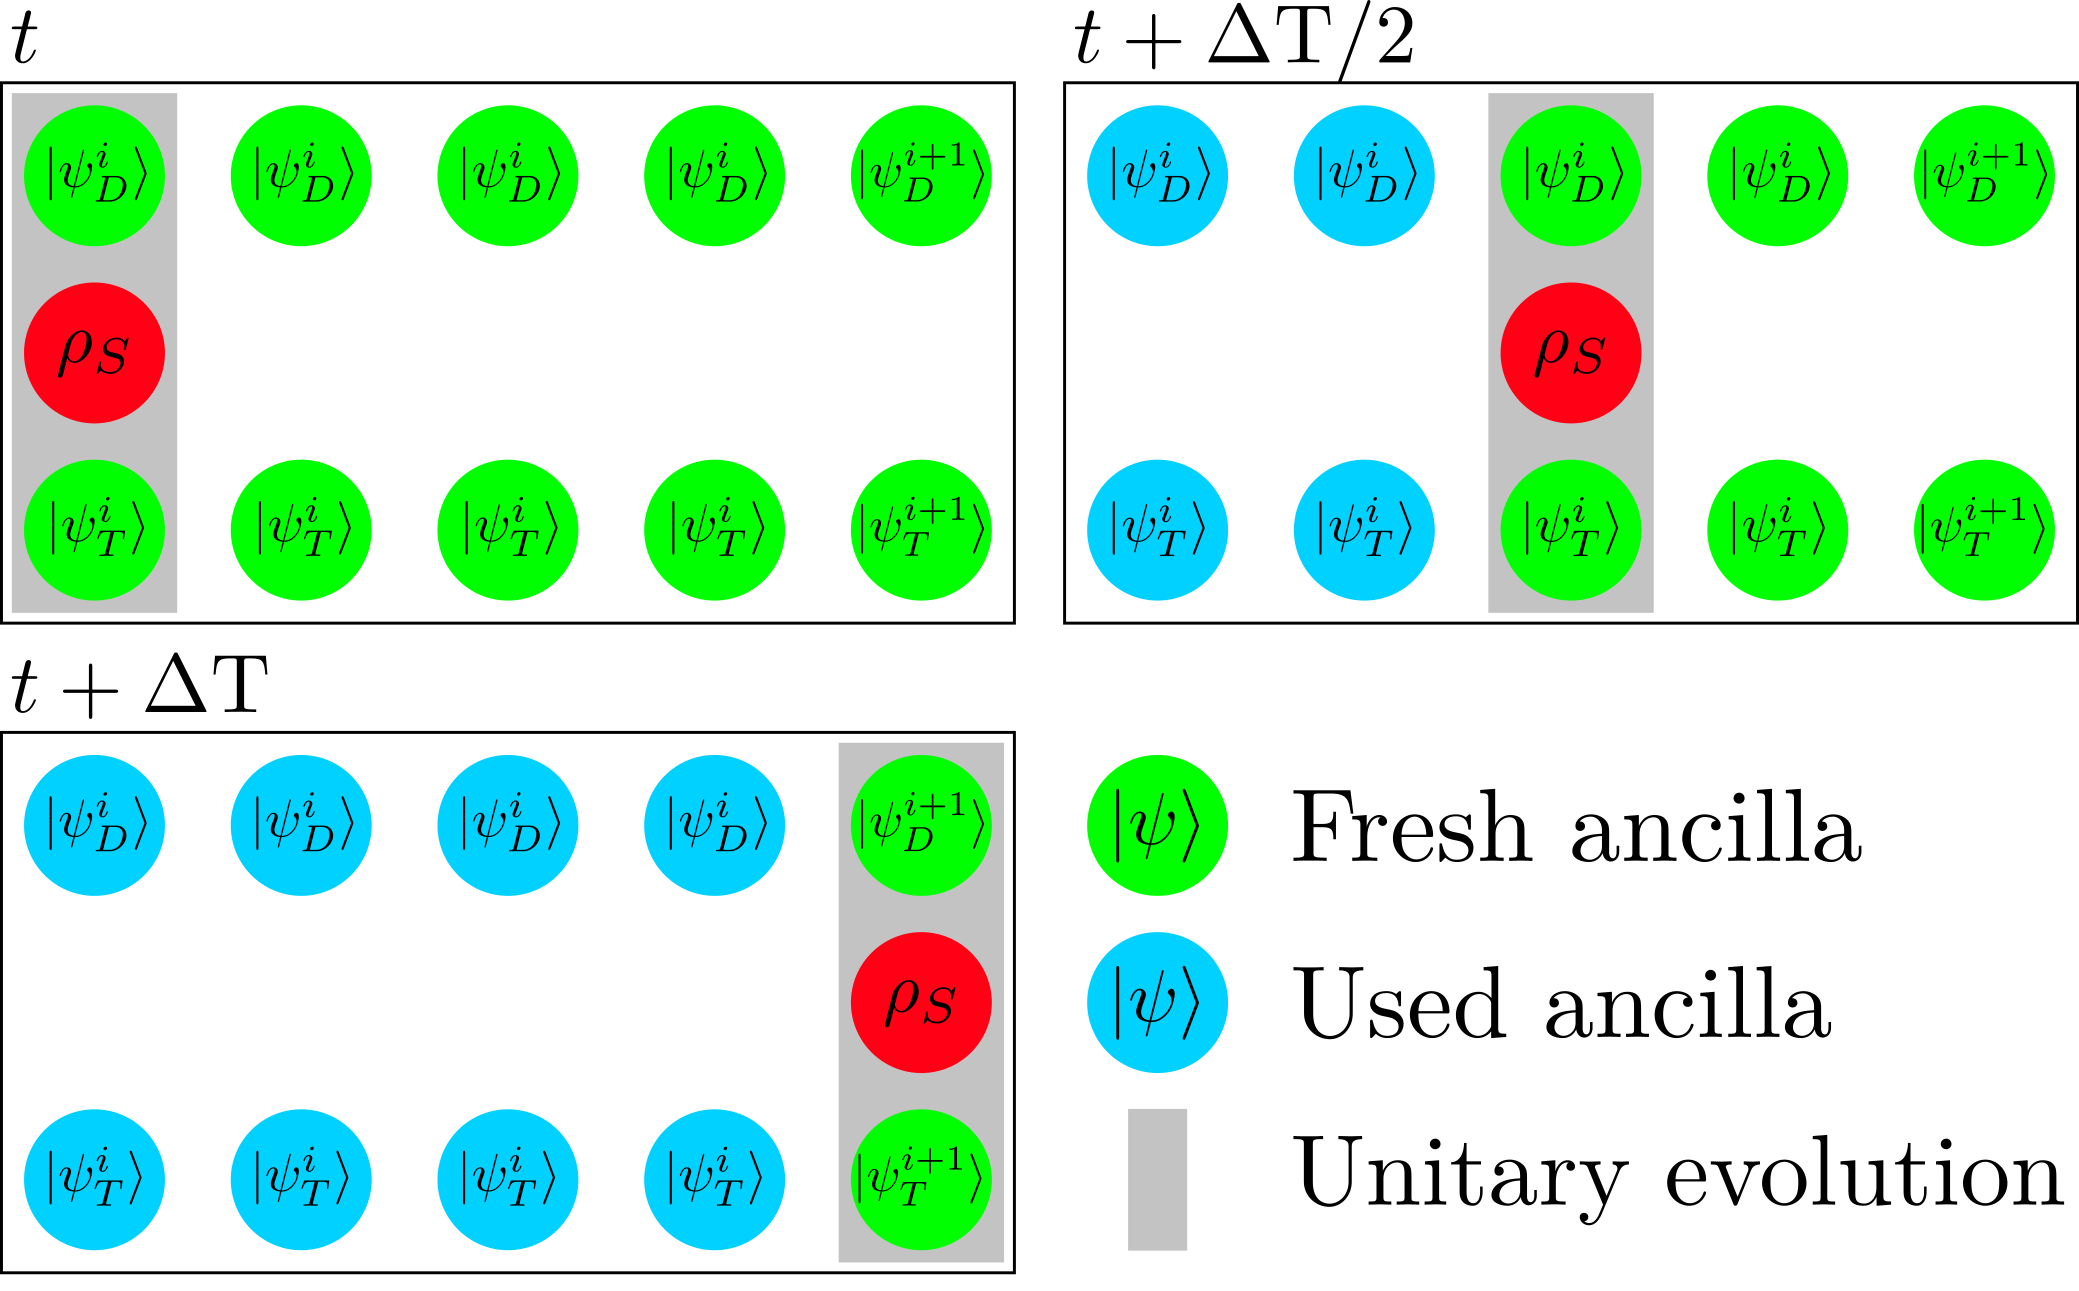
\includegraphics[width=0.7\textwidth]{img/collision_model}
	\caption{Collision model used in this work: Drive and Transducer are series of qubits interact once with the system and evolve the reduced density operator $\rho_S$. The qubit configuration can be changed in intervals of $\Delta \mathrm{T}$.}
	\label{collmodel}
\end{figure}


\chapter{Experimental Results}

\chapter{Summary and Outlook}

\bibliographystyle{plain}
\bibliography{biblio}

% Erklärung
\clearpage
\thispagestyle{empty}
\minisec{Erklärung}\vspace*{1.5em}

Hiermit erkläre ich, dass ich diese Arbeit im Rahmen der Betreuung am Institut
für Theoretische Physik ohne unzulässige Hilfe Dritter verfasst und alle Quellen als solche gekennzeichnet habe.

\vspace*{45em}

Felix Soest \par
Dresden, Monat 2021

\end{document}
